\chapter{Computational Study}\label{chapter:study}
xyz?

\section{Experimental Design}\label{sec:stu-experiment}
xyz?

\subsection{Framework Implementation}\label{sec:stu-implementation}
All experiments in this chapter run on a single, shared department server, Ubuntu 22.04 LTS, two Intel Xeon E5-2697A v4 CPUs at 2.60 GHz (16 cores each, 32 cores and 64 threads total) and 125 GB of RAM, with no GPU\@. DRISPI runs inside Docker containers (Docker 29.6.1) pinned to a disjoint CPU range with \texttt{--cpuset-cpus}, because other jobs share the same server, and every worker sets \texttt{OMP\_NUM\_THREADS}, \texttt{OPENBLAS\_NUM\_THREADS}, and \texttt{MKL\_NUM\_THREADS} to one; the pinned CPU count, not a library thread-pool default, therefore sets the framework's own parallelism budget.

The 100-instance, three-seed campaign behind Section~\ref{sec:stu-comparison} (300 runs, 7{,}200 seconds each) pins 32 of the server's 64 logical CPUs as four exclusive 8-core Docker containers, each split six DRI workers, one BG-AILS worker, and one SP worker, the \texttt{cores} block of \texttt{configs/final\_benchmark.yaml}. Runs are packed into waves ordered by instance size so that the three seeds of the largest instance, XL-n10001-k1570, never share a wave; the full campaign takes 75 waves and about 150 hours of wall-clock time.

Section~\ref{sec:fra-routing} introduces the four subsolvers and Section~\ref{sec:fra-sp} the Gurobi SC/SP step; this section fixes the concrete versions behind them. DRISPI targets Python 3.11, the version scikit-learn-extra's k-medoids implementation requires, with dependencies locked via \texttt{uv}: PyVRP 0.13.3, scikit-learn 1.8.0 (K-Means and agglomerative clustering), scikit-learn-extra 0.3.0 (k-medoids), scikit-fuzzy 0.5.0 (Fuzzy C-Means), gurobipy 13.0.1, and vrplib 2.1.0 for instance parsing. AILS-II, FILO, and FILO2 are vendored as git submodules pinned to a fixed commit each and compiled at image build time, rather than resolved from a floating branch, so a rebuild reproduces the exact binaries behind the results in Section~\ref{sec:stu-comparison}. The whole framework runs inside a Docker image built from this locked environment, so the software stack behind every reported run is fixed independently of the host it executes on.

\subsection{Dataset}\label{sec:stu-dataset}
Chapter~\ref{chapter:problem} introduces the XL instance set, the 100 \gls{cvrp} instances with which \citet{queirogaXLInstancesCapacitated2026} extend the 100-to-1{,}000-customer X set of \citet{uchoaNewBenchmarkInstances2017} up to 10{,}000 customers. \citet{queirogaXLInstancesCapacitated2026} generate every instance from the X set's own scheme: two-dimensional Euclidean coordinates on a $[0,1{,}000]\times[0,1{,}000]$ grid, with the depot Random, Central at (500, 500), or Eccentric at (0, 0); customers Random, Clustered, or Random-Clustered around a small number of seed points; demand drawn from one of seven distributions, from unitary demand (U) through four ranges of increasing width (1--10, 5--10, 1--100, 50--100) to a quadrant-dependent range (Q) and a mix of many small and few large demands (SL); and a target average route length $r$ drawn from one of seven bands, from ultra-short ($r \in [3,5]$) to ultra-long ($r \in [50,200]$). Vehicle capacity $Q$ and the vehicle count are chosen jointly so that a solution using the minimum feasible number of routes attains the target $r$. The instance name encodes both n and this minimum route count, for example XL-n4535-k1134 for the 4,535-customer instance with a 1,134-route lower bound; this $k$ is fixed by the benchmark set and unrelated to the decomposition subcluster count of the same name (Section~\ref{sec:fra-haos}), and solutions using more than $k$ routes remain feasible. Appendix~\ref{app:xl-results} lists the depot position, customer distribution, demand distribution, $Q$, and $r$ of every instance in the abbreviations just defined, alongside DRISPI's result.

\citet{queirogaXLInstancesCapacitated2026} establish an initial \gls{bks} for each instance from sixty runs of eight monolithic \gls{cvrp} solvers: AILS-II, FILO, FILO2, KGLSXXL, HGS-CVRP, SISRs, LKH-3, and OR-Tools. AILS-II alone supplies 93 of the 100 initial values, FILO2 six, and FILO one. Section~\ref{sec:stu-comparison} benchmarks DRISPI against the same eight solvers.

These initial values were a starting point rather than a permanent baseline. \citet{queirogaXLInstancesCapacitated2026} launch them alongside the CVRPLib \gls{bks} Challenge, a 30-day, community-run competition, opened January 12, 2026, in which any team can submit an improved feasible solution for an XL instance, verified automatically by the CVRPLib platform. By the current record\footnote{\url{https://galgos.inf.puc-rio.br/cvrplib/index.php/en/bks_challenge/score/instances}, accessed September 7, 2026.}, the challenge has improved 99 of the 100 initial values; XL-n1094-k157 is the only instance still at its initial value. Every gap reported in this chapter therefore uses the current \gls{bks} record as the baseline, not the initial values \citet{queirogaXLInstancesCapacitated2026} report.

\subsection{Repetitions}\label{sec:stu-repetitions}
DRISPI runs every one of the 100 XL instances three times, $S=3$, at the fixed seeds 10, 20, and 30, disclosed here for reproducibility, each run stopped after 7{,}200 seconds (120 minutes) of wall-clock time rather than at convergence. Each run is therefore a terminating simulation in the sense of \citet{lawSimulationModelingAnalysis2000}: a fixed initial condition, the first DRI iteration's decomposition and routing pass (Section~\ref{sec:fra-decomposition}), and a fixed stopping rule rather than a steady state. The replication method of \citet[ch.~9]{lawSimulationModelingAnalysis2000} therefore applies; neither warm-up deletion nor batch means do.

The interval sized below is conditional on the fixed 100-instance Queiroga XL set ($n$ from 1{,}048 to 10{,}001 customers, Section~\ref{sec:stu-dataset}): the instances are a design factor \citep{queirogaXLInstancesCapacitated2026}, not a sample from a superpopulation of \gls{cvrp} instances, so seed is the only randomness the design controls. With $\bar G$ the grand mean gap and $\bar\sigma^2$ the average per-instance seed variance, $\mathrm{Var}(\bar G) = \bar\sigma^2/(I \cdot S)$, $I=100$; an unconditional target would add a between-instance term that swamps the seed term and makes $S$ nearly irrelevant, so the conditional target is stated explicitly. The interval does not extend to the published baselines Section~\ref{sec:stu-comparison} compares against, each a single reported value per instance with no variance estimate of its own.

Independence across instances is asserted mechanistically rather than inferred from the pilot data: every run executes as a separate process with its own seeded random-number stream, and DRISPI shares no pool, cache, or global counter across instances (Chapter~\ref{chapter:framework}), so the $I \times S$ observations behind $\bar G$ are independent by construction.

The pilot campaign (three instances, four seeds each, five wall-clock marks per run) measured a root-mean-square per-instance seed standard deviation of 0.118 percentage points at the 7{,}200 second mark. The target margin was fixed in advance at $\pm 0.03$ percentage points, chosen to resolve the 0.02--0.06 pp effect sizes observed in earlier component A/B tests. Table~\ref{tab:seed-sizing} forecasts the standard error and normal-approximation 95\% half-width of $\bar G$ at this pilot sigma, $S$ from one to four, $I=100$. Every value of $S$ clears the target by a comfortable margin, so precision alone does not select $S=3$.

\begin{table}[htbp]
\centering
\caption{Forecast standard error and normal-approximation 95\% half-width of the set-level mean gap $\bar G$, at the pilot standard deviation of 0.118 pp per instance-seed and $I=100$ instances.}\label{tab:seed-sizing}
\begin{tabular}{@{}lrr@{}}
\toprule
$S$ & SE (pp) & Half-width (pp) \\
\midrule
1 & 0.0118 & 0.023 \\
2 & 0.0083 & 0.016 \\
3 & 0.0068 & 0.013 \\
4 & 0.0059 & 0.012 \\
\bottomrule
\end{tabular}
\end{table}

Three considerations beyond precision fix $S=3$. First, degrees of freedom: pooled within-instance degrees of freedom, $I(S-1)$, are zero at $S=1$ and admit no interval at all; at $S=3$ they are 200, reduced by Satterthwaite to approximately 138 given the pilot's heterogeneous variances (3.7-fold in standard deviation, 13.6-fold in variance), giving $t(0.975,138)\approx1.98$, close to the normal approximation above. Second, identifiability: at $S=2$ a discrepancy between two runs is measurable but not attributable; at $S=3$ a single anomalous replication can be isolated against the other two, a capacity the campaign exercised (Section~\ref{TODO}). Third, best-of-$S$ requires $S>1$ to be a nontrivial minimum, and the convention on this instance set, following \citet{queirogaXLInstancesCapacitated2026}, reports such a column.

The design already commits 300 runs, 7{,}200 seconds each, to four concurrent eight-core slices on the department server (Section~\ref{sec:stu-implementation}): 150 hours of wall-clock time, 4{,}800 core-hours. A fourth seed would add 100 more runs, about 1{,}600 core-hours, for a half-width gain from 0.013 to 0.012 pp, against a systematic batch effect of approximately 0.039 pp that two pilot campaigns differing only in execution environment showed, roughly three times the forecast $S=3$ half-width and identified in advance as the binding constraint on validity, not the replication count. \citet{johnsonTheoreticiansGuideExperimental2002} and \citet{barrDesigningReportingComputational1995} both argue for sizing a campaign against its dominant nuisance source rather than against statistical power alone; a fourth seed buys the latter on a term already dominated by the former.

Neyman allocation, assigning more replications to higher-variance instances, was evaluated against equal allocation at the same total budget. Despite the 13.6-fold variance spread across the pilot instances, it recovers only an 8.8\% reduction in the standard error of $\bar G$, so equal allocation, three seeds on every instance, was retained.

Two caveats qualify this design. The seed is a replication label, not a determinism guarantee: DRISPI's \texttt{ProcessPoolExecutor}-based worker pool schedules subcluster work non-deterministically, so two runs at the same seed are exchangeable replications rather than bitwise-reproducible runs. The best-of-$S$ statistic is an extreme-value statistic whose expectation depends on $S$, not comparable across publications using a different replication count; the interval above applies to the mean-over-seeds statistic $\bar G$ only, a distinction stated here so Section~\ref{sec:stu-comparison} can rely on it rather than restate it.

Realized seed variance and the per-seed breakdown appear in Section~\ref{TODO}; the paired Wilcoxon signed-rank tests with Holm correction on per-instance differences, following \citet{demsVarStatisticalComparisonsClassifiers}, are specified in Section~\ref{TODO}.

\subsection{Hyperparameters}\label{sec:stu-hyperparameters}
Show the hyperparameters used for the benchmark run. Explain the impact of the different hyperparameters on the performance.

\section{Results}\label{sec:stu-results}
Short introduction.

\subsection{Performance Comparison against State-of-the-Art Monolithic Solvers}\label{sec:stu-comparison}
Table~\ref{tab:solver-summary} compares DRISPI against the eight monolithic solvers \citet{queirogaXLInstancesCapacitated2026} benchmark on the 100 XL instances: AILS-II, FILO, FILO2, KGLSXXL, HGS-CVRP, SISRs, LKH-3, and OR-Tools. For every solver we recompute the percentage gap to the current official \gls{bks}, the record listed by the CVRPLib \gls{bks} Challenge (Section~\ref{sec:stu-dataset}), for both the mean-of-$N$ and best-of-$N$ cost the original paper reports ($N=60$ for the published solvers, $N=3$ for DRISPI), then average that per-instance gap over all 100 instances and, separately, over the fifty instances with fewer than 3,400 customers and the fifty with more, the split \citet{queirogaXLInstancesCapacitated2026} use for their own results table. Every gap in Table~\ref{tab:solver-summary} uses the current \gls{bks} as the denominator, including for the published solvers. \citet{queirogaXLInstancesCapacitated2026} report their own average gaps against the \gls{bks} at the time of publication, effectively AILS-II's own result for most instances, so those published averages are not comparable to the ones reported here. Appendix~\ref{app:xl-results} lists the per-instance detail behind DRISPI's two columns: instance characteristics, best cost, and gap, alongside both \gls{bks} references (Table~\ref{tab:xl-summary}).

\begin{longtable}{@{}lrrrrrr@{}}
\caption{Mean percentage gap to the current \gls{bks} across all 100 XL instances, split into the fifty instances with fewer than 3,400 customers and the fifty with more, following \citet{queirogaXLInstancesCapacitated2026}. Mean-of-$N$ averages the sixty runs per published solver (three seeds for DRISPI); best-of-$N$ is the minimum. Sorted by ascending mean-of-$N$ gap over all instances.}\label{tab:solver-summary}\\
\toprule
& \multicolumn{3}{c}{Mean-of-$N$ Gap (\%)} & \multicolumn{3}{c}{Best-of-$N$ Gap (\%)} \\
\cmidrule(lr){2-4} \cmidrule(lr){5-7}
Solver & All & $n<3{,}400$ & $n>3{,}400$ & All & $n<3{,}400$ & $n>3{,}400$ \\
\midrule
\endfirsthead
\toprule
& \multicolumn{3}{c}{Mean-of-$N$ Gap (\%)} & \multicolumn{3}{c}{Best-of-$N$ Gap (\%)} \\
\cmidrule(lr){2-4} \cmidrule(lr){5-7}
Solver & All & $n<3{,}400$ & $n>3{,}400$ & All & $n<3{,}400$ & $n>3{,}400$ \\
\midrule
\endhead
\bottomrule
\endfoot
\bottomrule
\endlastfoot
AILS-II & +0.16 & +0.14 & +0.18 & +0.09 & +0.06 & +0.12 \\
FILO2 & +0.29 & +0.29 & +0.30 & +0.20 & +0.17 & +0.23 \\
\gls{drispi} & +0.31 & +0.24 & +0.37 & +0.28 & +0.21 & +0.34 \\
FILO & +0.33 & +0.31 & +0.36 & +0.24 & +0.19 & +0.28 \\
SISRs & +0.58 & +0.49 & +0.68 & +0.42 & +0.30 & +0.55 \\
KGLSXXL & +1.09 & +0.87 & +1.31 & +0.88 & +0.64 & +1.12 \\
HGS-CVRP & +1.45 & +0.83 & +2.06 & +1.20 & +0.60 & +1.80 \\
LKH-3 ($n = 90$) & +6.75 & +5.01 & +8.92 & +5.56 & +4.03 & +7.48 \\
OR-Tools & +6.90 & +6.77 & +7.03 & +5.63 & +5.43 & +5.83 \\

\end{longtable}

Mean-of-$N$ is the primary comparison in Table~\ref{tab:solver-summary}, because DRISPI's mean-of-3 and each published solver's mean-of-60 both estimate the same population quantity, the expected cost of a single run, and are just averages over different sample sizes. Best-of-$N$ is not: it is the minimum of three draws for DRISPI against the minimum of sixty for every published solver, a sampling budget 20 times larger, which mechanically favors the columns with more draws. Sampling one of DRISPI's own three seed costs at a time gives an expected best-of-1 gap equal to the mean-of-3 gap, 0.309\%; the average of the smaller cost in each of the three retained seed pairs gives a best-of-2 gap of 0.286\%; the actual three-seed minimum gives the best-of-3 gap of 0.277\%, already reported in Table~\ref{tab:solver-summary}. The marginal gain is 0.022 pp from the first extra sample and 0.009 pp from the second. AILS-II, FILO2, FILO, SISRs, KGLSXXL, and HGS-CVRP gain 0.07, 0.09, 0.10, 0.16, 0.21, and 0.25 pp respectively between their own mean-of-60 and best-of-60 columns, larger reductions from many more repetitions. DRISPI's mean per-instance seed standard deviation is 0.035 pp, so additional seeds narrow its best column by less than they narrow a higher-variance baseline's. This produces the rank inversion in Table~\ref{tab:solver-summary}: DRISPI ranks third by mean-of-$N$ and fourth by best-of-$N$, without a change in the underlying solution quality; the difference is which column rewards low run-to-run variance and which rewards a wide sampling budget. Best-of-$N$ is reported to match the published solvers' own headline metric, not as the primary comparison.

The means in Table~\ref{tab:solver-summary} do not establish whether an observed difference is real rather than an artifact of the 100 sampled instances. We tested DRISPI's mean-of-3 and best-of-3 columns against the corresponding column of five of the eight published solvers, AILS-II, FILO2, FILO, SISRs, and HGS-CVRP, with the paired Wilcoxon signed-rank test \citep{demsVarStatisticalComparisonsClassifiers}, treating the 100 instances as matched pairs, and controlled the family-wise error rate across the resulting ten tests with the Holm step-down correction \citep{demsVarStatisticalComparisonsClassifiers}. KGLSXXL, LKH-3, and OR-Tools are omitted: their gaps in Table~\ref{tab:solver-summary} are large enough that the paired comparison would not be informative. DRISPI is significantly worse than AILS-II on both metrics (best-of-$N$: +0.188 pp, DRISPI ahead on one of 100 instances, Holm-corrected $p=5.5\times10^{-17}$; mean-of-$N$: +0.150 pp, DRISPI ahead on seven of 100, $p=2.5\times10^{-16}$) and significantly better than SISRs on both (best-of-$N$: $-0.148$ pp, $p=1.1\times10^{-10}$; mean-of-$N$: $-0.274$ pp, $p=2.4\times10^{-16}$). DRISPI is significantly better than HGS-CVRP on both metrics as well, by a wider margin (best-of-$N$: $-0.924$ pp, DRISPI ahead on 96 of 100 instances, $p=6.4\times10^{-17}$; mean-of-$N$: $-1.139$ pp, DRISPI ahead on all 100 instances, $p=3.9\times10^{-17}$). Against FILO, neither metric reaches significance (best-of-$N$: +0.040 pp, $p=0.51$; mean-of-$N$: $-0.025$ pp, $p=0.34$): the two are indistinguishable at this sample size. Against FILO2, the two metrics disagree: DRISPI is significantly worse on best-of-$N$ (+0.074 pp, $p=0.0033$) but not on mean-of-$N$ (+0.015 pp, $p=0.51$), the primary comparison. The 0.015 pp mean-of-$N$ difference against FILO2 does not survive correction for multiple testing and is not a demonstrated gap.

\begin{figure}[H]
\centering
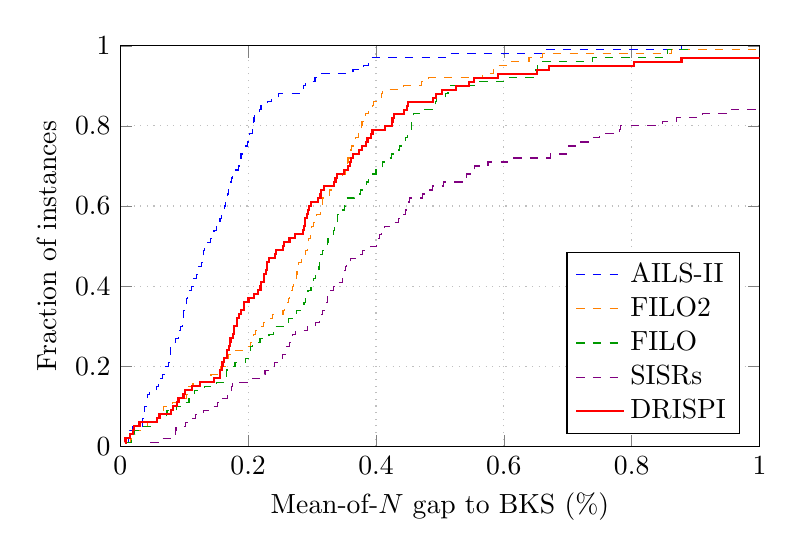
\begin{tikzpicture}
\begin{axis}[
    width=0.8\textwidth, height=0.55\textwidth,
    xlabel={Mean-of-$N$ gap to BKS (\%)},
    ylabel={Fraction of instances},
    xmin=0, xmax=1,
    ymin=0, ymax=1,
    legend pos=south east,
    legend cell align=left,
    grid=major,
    grid style={dotted, gray!50},
]
\addplot+[const plot mark left, no markers, dashed, thin, color=blue] coordinates {(0.0079,0.0100) (0.0131,0.0200) (0.0139,0.0300) (0.0151,0.0400) (0.0192,0.0500) (0.0348,0.0600) (0.0349,0.0700) (0.0359,0.0800) (0.0378,0.0900) (0.0385,0.1000) (0.0412,0.1100) (0.0421,0.1200) (0.0426,0.1300) (0.0455,0.1400) (0.0560,0.1500) (0.0599,0.1600) (0.0638,0.1700) (0.0661,0.1800) (0.0690,0.1900) (0.0690,0.2000) (0.0755,0.2100) (0.0772,0.2200) (0.0788,0.2300) (0.0789,0.2400) (0.0791,0.2500) (0.0847,0.2600) (0.0862,0.2700) (0.0905,0.2800) (0.0929,0.2900) (0.0940,0.3000) (0.0968,0.3100) (0.0985,0.3200) (0.0991,0.3300) (0.0992,0.3400) (0.1010,0.3500) (0.1032,0.3600) (0.1038,0.3700) (0.1050,0.3800) (0.1059,0.3900) (0.1109,0.4000) (0.1139,0.4100) (0.1152,0.4200) (0.1196,0.4300) (0.1223,0.4400) (0.1228,0.4500) (0.1273,0.4600) (0.1285,0.4700) (0.1309,0.4800) (0.1309,0.4900) (0.1318,0.5000) (0.1322,0.5100) (0.1406,0.5200) (0.1432,0.5300) (0.1466,0.5400) (0.1499,0.5500) (0.1544,0.5600) (0.1560,0.5700) (0.1580,0.5800) (0.1623,0.5900) (0.1625,0.6000) (0.1644,0.6100) (0.1648,0.6200) (0.1682,0.6300) (0.1693,0.6400) (0.1696,0.6500) (0.1724,0.6600) (0.1743,0.6700) (0.1757,0.6800) (0.1772,0.6900) (0.1851,0.7000) (0.1864,0.7100) (0.1875,0.7200) (0.1888,0.7300) (0.1908,0.7400) (0.1955,0.7500) (0.1991,0.7600) (0.2004,0.7700) (0.2021,0.7800) (0.2067,0.7900) (0.2076,0.8000) (0.2081,0.8100) (0.2092,0.8200) (0.2105,0.8300) (0.2181,0.8400) (0.2201,0.8500) (0.2304,0.8600) (0.2371,0.8700) (0.2476,0.8800) (0.2797,0.8900) (0.2861,0.9000) (0.2895,0.9100) (0.3047,0.9200) (0.3120,0.9300) (0.3641,0.9400) (0.3806,0.9500) (0.3879,0.9600) (0.3888,0.9700) (0.5124,0.9800) (0.6627,0.9900) (0.8781,1.0000)};
\addlegendentry{AILS-II}

\addplot+[const plot mark left, no markers, dashed, thin, color=orange] coordinates {(0.0119,0.0100) (0.0168,0.0200) (0.0193,0.0300) (0.0199,0.0400) (0.0312,0.0500) (0.0423,0.0600) (0.0567,0.0700) (0.0599,0.0800) (0.0670,0.0900) (0.0682,0.1000) (0.0812,0.1100) (0.0983,0.1200) (0.1034,0.1300) (0.1054,0.1400) (0.1054,0.1500) (0.1138,0.1600) (0.1416,0.1700) (0.1419,0.1800) (0.1526,0.1900) (0.1565,0.2000) (0.1648,0.2100) (0.1667,0.2200) (0.1694,0.2300) (0.1766,0.2400) (0.1943,0.2500) (0.2035,0.2600) (0.2070,0.2700) (0.2091,0.2800) (0.2116,0.2900) (0.2177,0.3000) (0.2244,0.3100) (0.2345,0.3200) (0.2381,0.3300) (0.2546,0.3400) (0.2574,0.3500) (0.2615,0.3600) (0.2629,0.3700) (0.2646,0.3800) (0.2675,0.3900) (0.2690,0.4000) (0.2713,0.4100) (0.2718,0.4200) (0.2760,0.4300) (0.2764,0.4400) (0.2787,0.4500) (0.2793,0.4600) (0.2832,0.4700) (0.2883,0.4800) (0.2895,0.4900) (0.2931,0.5000) (0.2938,0.5100) (0.2949,0.5200) (0.2977,0.5300) (0.2984,0.5400) (0.2996,0.5500) (0.3025,0.5600) (0.3063,0.5700) (0.3066,0.5800) (0.3132,0.5900) (0.3156,0.6000) (0.3160,0.6100) (0.3162,0.6200) (0.3274,0.6300) (0.3275,0.6400) (0.3337,0.6500) (0.3353,0.6600) (0.3359,0.6700) (0.3480,0.6800) (0.3517,0.6900) (0.3535,0.7000) (0.3550,0.7100) (0.3562,0.7200) (0.3579,0.7300) (0.3583,0.7400) (0.3623,0.7500) (0.3664,0.7600) (0.3676,0.7700) (0.3725,0.7800) (0.3760,0.7900) (0.3774,0.8000) (0.3782,0.8100) (0.3837,0.8200) (0.3838,0.8300) (0.3890,0.8400) (0.3951,0.8500) (0.3961,0.8600) (0.4034,0.8700) (0.4089,0.8800) (0.4096,0.8900) (0.4427,0.9000) (0.4715,0.9100) (0.4826,0.9200) (0.5665,0.9300) (0.5832,0.9400) (0.5897,0.9500) (0.6047,0.9600) (0.6394,0.9700) (0.6600,0.9800) (0.8621,0.9900) (1.0528,1.0000)};
\addlegendentry{FILO2}

\addplot+[const plot mark left, no markers, dashed, thin, color=green!60!black] coordinates {(0.0090,0.0100) (0.0179,0.0200) (0.0200,0.0300) (0.0225,0.0400) (0.0330,0.0500) (0.0529,0.0600) (0.0575,0.0700) (0.0720,0.0800) (0.0732,0.0900) (0.0886,0.1000) (0.0979,0.1100) (0.1076,0.1200) (0.1090,0.1300) (0.1155,0.1400) (0.1315,0.1500) (0.1507,0.1600) (0.1642,0.1700) (0.1657,0.1800) (0.1658,0.1900) (0.1670,0.2000) (0.1795,0.2100) (0.1963,0.2200) (0.2024,0.2300) (0.2034,0.2400) (0.2044,0.2500) (0.2075,0.2600) (0.2186,0.2700) (0.2327,0.2800) (0.2394,0.2900) (0.2417,0.3000) (0.2560,0.3100) (0.2628,0.3200) (0.2687,0.3300) (0.2756,0.3400) (0.2848,0.3500) (0.2874,0.3600) (0.2902,0.3700) (0.2910,0.3800) (0.2936,0.3900) (0.2984,0.4000) (0.2995,0.4100) (0.3016,0.4200) (0.3058,0.4300) (0.3089,0.4400) (0.3109,0.4500) (0.3113,0.4600) (0.3120,0.4700) (0.3136,0.4800) (0.3159,0.4900) (0.3219,0.5000) (0.3236,0.5100) (0.3250,0.5200) (0.3294,0.5300) (0.3334,0.5400) (0.3349,0.5500) (0.3386,0.5600) (0.3396,0.5700) (0.3401,0.5800) (0.3439,0.5900) (0.3503,0.6000) (0.3529,0.6100) (0.3538,0.6200) (0.3670,0.6300) (0.3759,0.6400) (0.3806,0.6500) (0.3850,0.6600) (0.3890,0.6700) (0.3939,0.6800) (0.4000,0.6900) (0.4099,0.7000) (0.4103,0.7100) (0.4174,0.7200) (0.4249,0.7300) (0.4329,0.7400) (0.4364,0.7500) (0.4456,0.7600) (0.4465,0.7700) (0.4499,0.7800) (0.4519,0.7900) (0.4554,0.8000) (0.4562,0.8100) (0.4581,0.8200) (0.4586,0.8300) (0.4744,0.8400) (0.4907,0.8500) (0.4933,0.8600) (0.4945,0.8700) (0.5081,0.8800) (0.5126,0.8900) (0.5157,0.9000) (0.5594,0.9100) (0.6033,0.9200) (0.6471,0.9300) (0.6493,0.9400) (0.6524,0.9500) (0.6597,0.9600) (0.7394,0.9700) (0.8492,0.9800) (0.8555,0.9900) (0.8904,1.0000)};
\addlegendentry{FILO}

\addplot+[const plot mark left, no markers, dashed, thin, color=violet] coordinates {(0.0467,0.0100) (0.0592,0.0200) (0.0802,0.0300) (0.0869,0.0400) (0.0872,0.0500) (0.1024,0.0600) (0.1055,0.0700) (0.1171,0.0800) (0.1302,0.0900) (0.1440,0.1000) (0.1523,0.1100) (0.1569,0.1200) (0.1678,0.1300) (0.1686,0.1400) (0.1734,0.1500) (0.1749,0.1600) (0.2033,0.1700) (0.2192,0.1800) (0.2265,0.1900) (0.2410,0.2000) (0.2411,0.2100) (0.2482,0.2200) (0.2534,0.2300) (0.2586,0.2400) (0.2600,0.2500) (0.2648,0.2600) (0.2692,0.2700) (0.2701,0.2800) (0.2744,0.2900) (0.2924,0.3000) (0.3058,0.3100) (0.3118,0.3200) (0.3153,0.3300) (0.3168,0.3400) (0.3219,0.3500) (0.3222,0.3600) (0.3239,0.3700) (0.3241,0.3800) (0.3255,0.3900) (0.3336,0.4000) (0.3374,0.4100) (0.3474,0.4200) (0.3495,0.4300) (0.3507,0.4400) (0.3520,0.4500) (0.3544,0.4600) (0.3607,0.4700) (0.3718,0.4800) (0.3791,0.4900) (0.3911,0.5000) (0.4002,0.5100) (0.4034,0.5200) (0.4054,0.5300) (0.4082,0.5400) (0.4127,0.5500) (0.4291,0.5600) (0.4358,0.5700) (0.4389,0.5800) (0.4460,0.5900) (0.4479,0.6000) (0.4502,0.6100) (0.4528,0.6200) (0.4731,0.6300) (0.4776,0.6400) (0.4891,0.6500) (0.5051,0.6600) (0.5345,0.6700) (0.5417,0.6800) (0.5513,0.6900) (0.5548,0.7000) (0.5752,0.7100) (0.6060,0.7200) (0.6725,0.7300) (0.7003,0.7400) (0.7011,0.7500) (0.7163,0.7600) (0.7326,0.7700) (0.7492,0.7800) (0.7814,0.7900) (0.7820,0.8000) (0.8477,0.8100) (0.8696,0.8200) (0.9101,0.8300) (0.9505,0.8400) (1.0131,0.8500) (1.0203,0.8600) (1.0754,0.8700) (1.1176,0.8800) (1.1189,0.8900) (1.1438,0.9000) (1.2760,0.9100) (1.3285,0.9200) (1.3289,0.9300) (1.6629,0.9400) (1.8294,0.9500) (1.9515,0.9600) (2.0976,0.9700) (2.2883,0.9800) (2.3910,0.9900) (3.4960,1.0000)};
\addlegendentry{SISRs}

\addplot+[const plot mark left, no markers, solid, thick, color=red] coordinates {(0.0075,0.0100) (0.0083,0.0200) (0.0155,0.0300) (0.0200,0.0400) (0.0211,0.0500) (0.0301,0.0600) (0.0570,0.0700) (0.0615,0.0800) (0.0791,0.0900) (0.0830,0.1000) (0.0882,0.1100) (0.0912,0.1200) (0.0989,0.1300) (0.1017,0.1400) (0.1126,0.1500) (0.1251,0.1600) (0.1462,0.1700) (0.1555,0.1800) (0.1561,0.1900) (0.1597,0.2000) (0.1599,0.2100) (0.1620,0.2200) (0.1669,0.2300) (0.1671,0.2400) (0.1704,0.2500) (0.1722,0.2600) (0.1726,0.2700) (0.1764,0.2800) (0.1777,0.2900) (0.1779,0.3000) (0.1826,0.3100) (0.1830,0.3200) (0.1859,0.3300) (0.1883,0.3400) (0.1933,0.3500) (0.1934,0.3600) (0.2005,0.3700) (0.2086,0.3800) (0.2153,0.3900) (0.2195,0.4000) (0.2199,0.4100) (0.2249,0.4200) (0.2251,0.4300) (0.2275,0.4400) (0.2291,0.4500) (0.2296,0.4600) (0.2329,0.4700) (0.2420,0.4800) (0.2436,0.4900) (0.2548,0.5000) (0.2560,0.5100) (0.2648,0.5200) (0.2739,0.5300) (0.2864,0.5400) (0.2871,0.5500) (0.2885,0.5600) (0.2887,0.5700) (0.2918,0.5800) (0.2937,0.5900) (0.2948,0.6000) (0.2984,0.6100) (0.3098,0.6200) (0.3133,0.6300) (0.3140,0.6400) (0.3183,0.6500) (0.3344,0.6600) (0.3367,0.6700) (0.3387,0.6800) (0.3500,0.6900) (0.3567,0.7000) (0.3595,0.7100) (0.3614,0.7200) (0.3644,0.7300) (0.3734,0.7400) (0.3784,0.7500) (0.3847,0.7600) (0.3868,0.7700) (0.3926,0.7800) (0.3945,0.7900) (0.4139,0.8000) (0.4255,0.8100) (0.4257,0.8200) (0.4282,0.8300) (0.4444,0.8400) (0.4484,0.8500) (0.4499,0.8600) (0.4895,0.8700) (0.4936,0.8800) (0.5033,0.8900) (0.5246,0.9000) (0.5459,0.9100) (0.5533,0.9200) (0.5910,0.9300) (0.6524,0.9400) (0.6709,0.9500) (0.8039,0.9600) (0.8778,0.9700) (1.1692,0.9800) (1.1766,0.9900) (1.6826,1.0000)};
\addlegendentry{DRISPI}

\end{axis}
\end{tikzpicture}
\caption{Empirical cumulative distribution of the mean-of-$N$ gap to the current BKS, for the five solvers with a mean-of-$N$ gap below one percent in Table~\ref{tab:solver-summary}.}\label{fig:gap-ecdf}
\end{figure}

Figure~\ref{fig:gap-ecdf} shows why the Table~\ref{tab:solver-summary} means understate DRISPI's typical result and its tail at once: DRISPI's mean-of-3 gap has a mean of 0.309\% against a median of 0.255\% (interquartile range 0.172\%--0.380\%, ninetieth percentile 0.527\%, maximum 1.683\%), a right-skewed distribution in which most instances sit below the mean and a short tail sits well above it. DRISPI's curve tracks above FILO2's up to a gap of about 0.3\% (61\% of instances at or below that gap, against 55\% for FILO2) and falls below it from 0.4\% (79\% against 86\%), the crossover the non-significant paired mean-of-$N$ test against FILO2 allows: DRISPI wins on the tighter half of the distribution and loses on the wider half. Against FILO, DRISPI's curve stays at or above FILO's over the range shown, consistent with the near-even 53-of-100 split in the paired test.

Two individual results do not appear in any aggregate. On XL-n4535-k1134, DRISPI's best-of-3 cost of 1,203,553 is below the initial \gls{bks} of 1,203,566 \citet{queirogaXLInstancesCapacitated2026} reported at publication. On XL-n1094-k157, DRISPI's best-of-3 cost matches both the initial and the current \gls{bks} exactly, at 112,431. Across all 100 instances, DRISPI's best-of-3 cost matches or beats AILS-II's mean-of-60 on 12 instances (Appendix~\ref{app:xl-results}, Table~\ref{tab:xl-summary}).

\subsection{Performance by Instance Characteristics}\label{sec:stu-characteristics}
Show how DRISPI performs by instance characteristics. This should be a simple plot showing the performance by instance size, depot position, customer distribution, and demand distribution.

\subsection{HAOS Weights}\label{sec:stu-haos}
Investigate how HAOS weights are converging and if there are obvious tendencies. Interpret the results. 

Are some HAOS levels converging always to the same result? Are some HAOS levels always converging in a similar way subject to the instance characteristics? Whats the variance in HAOS weight convergence? Do they differ a lot from seed to seed and are sensitive to randomness?

Are the results interpretable in general?

\subsection{Convergence Behavior}\label{sec:stu-convergence}
Show how the convergence behavior is like for DRISPI by wallclock time and iterations. Use this chapter to also investigate improvement sources (quantitatively and qualitatively).

\section{Limitations}\label{sec:stu-limitations}
Lay out the limitations of the study. 

It should include the difficulty of comparing single-threaded monolithic solvers to the parallelized framework (CPU time vs. wallclock time, different hardware, etc.).

Also mention limitations and variations during the run when it comes to harware and number of seeds. Computation was a limiting factor here and definitely influenced performance.

Also mention that DRISPI's online learning approach obviously benefits from longer runtimes, especially for larger instances (as you can see the low number of iterations there, and that HAOS weights havent converged yet). This is also true for other instances, but especially the large and long-route ones would profit from HAOS convergence.